\scanpage{72}\mspage{71}

For what follows, we must pay attention to whether the axioms are going to pass to subcountries. Let us all the same introduce the definition in due form

% fig-definition: the raised word and its full hooked connector, with adjoining text once.
\figure{\begin{tikzpicture}[x=1cm,y=1cm]
\node[anchor=west] at (0,0) {\uline{Definition 1} We call a};
\node[anchor=west] at (7.4,0) {\uline{subcountry}};
\node[anchor=west] at (9.4,0.8) {\inserted{[\uline{full}]}};
\draw[line width=.55pt] (8.45,.48) .. controls (8.0,.28) and (10.9,.22) .. (11.35,.1) .. controls (11.85,.02) and (11.9,-.12) .. (12.0,-.23) .. controls (12.17,.03) and (12.28,.37) .. (12.31,.55);
\node[anchor=west] at (0,-1.05) {of the country $\unsure{\rlap{$\deleted{\mathcal F}$}\mathcal C|\mathcal C|\mathscr C|\mathbb C}=(\mathcal F,\leq,\preceq)$, \unsure{any|\deleted{any}}};
\node[anchor=west] at (0,-1.85) {subset which \unsure{satisfy|satisfies} the conditions};
\end{tikzpicture}}

% fig-a-insertions: correspond joins the physical line-end hyphen under convention 7; both insertion arms remain.
\figure{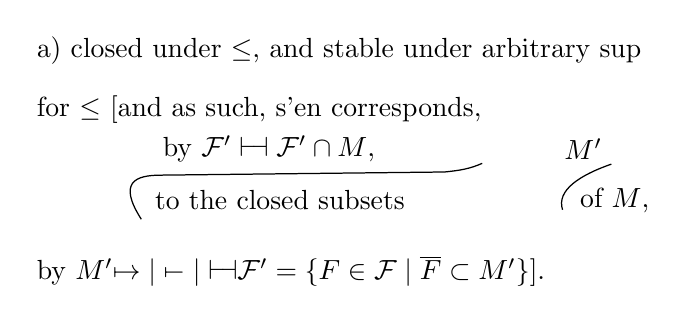
\begin{tikzpicture}[x=1cm,y=1cm]
\node[anchor=west] at (0,0) {a) closed under $\leq$, and stable under arbitrary sup};
\node[anchor=west] at (0,-.75) {for $\leq$ [and as such, s'en corresponds,};
\node[anchor=west] at (1.5,-1.9) {to the closed subsets};
\node[anchor=west] at (6.9,-1.9) {of $M$,};
\node[anchor=west] at (1.6,-1.25) {\inserted{by $\mathcal F'\mathrel{\vdash\joinrel\dashv}\mathcal F'\cap M$,}};
\node[anchor=west] at (6.7,-1.25) {\inserted{$M'$}};
\draw[line width=.45pt] (1.45,-2.14) .. controls (1.15,-1.67) and (1.37,-1.58) .. (1.7,-1.58) -- (5.3,-1.54) .. controls (5.5,-1.52) and (5.62,-1.50) .. (5.78,-1.43);
\draw[line width=.45pt] (6.8,-2.02) .. controls (6.72,-1.77) and (7.02,-1.58) .. (7.42,-1.44);
\node[anchor=west] at (0,-2.8) {by $M'\unsure{\mapsto|\mathrel{\mapstochar\relbar}|\mathrel{\vdash\joinrel\dashv}}\mathcal F'=\{F\in\mathcal F\mid\overline F\subset M'\}$].};
\end{tikzpicture}}

% slanted left margin; the terminal close is covered by root crop a05.
\margin{I do not know whether one should take arbitrary sup (strict \unsure{condition}) \deleted{\unsure{and}} or else finite sup only \unsure{(broad condition)|(broad condition)}}

% fig-b-correction: replacement above the cancelled clause; crossed/curling mark after M.
\figure{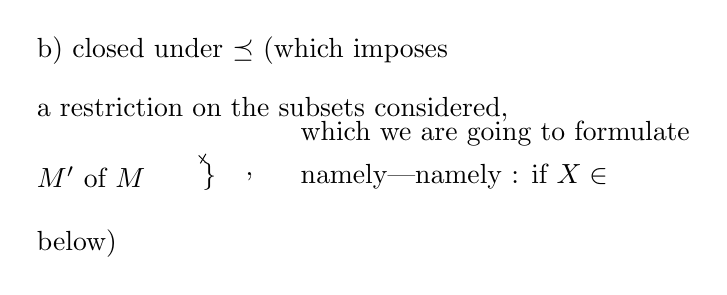
\begin{tikzpicture}[x=1cm,y=1cm]
\node[anchor=west] at (0,0) {b) closed under $\preceq$ (which imposes};
\node[anchor=west] at (0,-.75) {a restriction on the subsets considered,};
\node[anchor=west] at (0,-1.6) {$M'$ of $M$};
% fig-b-curled-mark: curled stroke with a small crossing at its head.
\node[anchor=west] at (2.1,-1.6) {\unsure{\}}};
\draw[line width=.35pt] (2.18,-1.33) -- (2.28,-1.43);
\draw[line width=.35pt] (2.20,-1.43) -- (2.27,-1.31);
\node[anchor=west] at (2.65,-1.6) {,};
\node[anchor=west] at (3.35,-1.6) {\deleted{\unsure{namely|namely} : if $X\in$}};
\node[anchor=west] at (3.35,-1.05) {\inserted{which we are going to formulate}};
\node[anchor=west] at (0,-2.45) {below)};
\end{tikzpicture}}

% fig-marginal-c: marginal continuation above C6; labels occur only here.
\figure{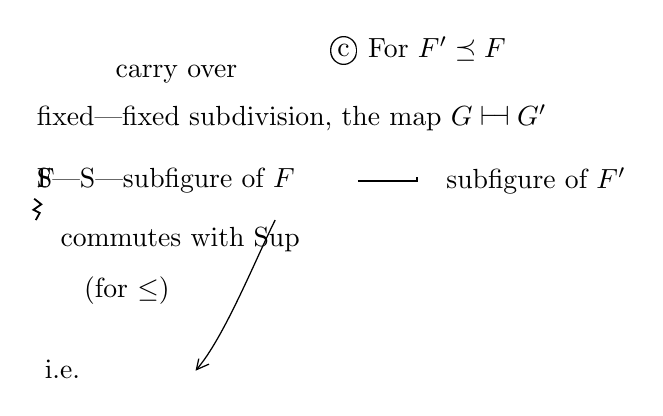
\begin{tikzpicture}[x=1cm,y=1cm]
\node[anchor=west] at (1.0,.55) {carry over};
\node[anchor=west] at (3.7,.85) {\textcircled{c} For $F'\preceq F$};
\node[anchor=west] at (0,0) {\unsure{fixed|fixed} subdivision, the map $G\mathrel{\vdash\joinrel\dashv}G'$};
% The worked initial is ONE letter position, including the lower residual strokes.
\node[anchor=west] at (0,-.8) {\unsure{\rlap{\deleted{F}}S|S|s}ubfigure of $F$};
\draw[line width=.65pt] (.09,-1.03) -- (.18,-1.10) -- (.08,-1.17) -- (.16,-1.21) -- (.11,-1.30);
% fig-c-headless-link: horizontal stroke with a very short raised right endpoint, no arrowhead.
\draw[line width=.6pt] (4.2,-.8) -- (4.95,-.8) -- (4.95,-.75);
\node[anchor=west] at (5.2,-.8) {subfigure of $F'$};
\node[anchor=west] at (.3,-1.55) {commutes with Sup};
\node[anchor=west] at (.6,-2.2) {(for $\leq$)};
\node[anchor=west] at (.1,-3.2) {i.e.};
% A distinct pointer descends leftward from the aux region.
\draw[line width=.45pt] (3.15,-1.3) .. controls (2.9,-1.8) and (2.5,-2.8) .. (2.15,-3.2);
\draw[line width=.45pt] (2.18,-3.06) -- (2.15,-3.2) -- (2.31,-3.13);
\end{tikzpicture}}

% diagram: C6-group. Diagrams remain diagrams; the two side rules, detached
% points and oblique gloss keep their relative positions. No text is repeated.
\diagram{\begin{tikzpicture}[x=1cm,y=1cm]
\node[anchor=west] at (0,0) {\uline{C6}};
\node[anchor=west] at (2.15,0) {Let};
\node at (4.05,-1.45) {\begin{tikzcd}[ampersand replacement=\&,column sep=1.6em,row sep=1.5em]
F' \arrow[r,phantom,"{\preceq}" description] \& F \arrow[d,phantom,"{\rotatebox{90}{$\leq$}}" description] \\
\& G
\end{tikzcd}};
\node[anchor=west] at (7.90,-1.15) {in $\mathcal F$};
\fill (2.01,-.88) circle (.012);
\fill (2.08,-.93) circle (.012);
\draw[line width=.4pt] (-.30,-.18) .. controls (-.27,-1.92) and (-.34,-3.62) .. (-.19,-4.78);
% slanted; the long rule is not treated as cancellation of this gloss.
\node[anchor=west,rotate=44,align=left] at (-2.00,-2.25) {symm\unsure{e|e}tric\\in $\leq,\preceq$};
\fill (-.46,-2.12) circle (.012);
\node[anchor=west] at (0,-3.05) {\textcircled{a} Then there exists a unique $H\in\mathcal F$ \unsure{with|or}};
\node at (4.10,-4.86) {\begin{tikzcd}[ampersand replacement=\&,column sep=1.6em,row sep=1.5em]
F' \arrow[r,phantom,"{\preceq}" description] \arrow[d,phantom,"{\rotatebox{90}{$\leq$}}" description] \& F \arrow[d,phantom,"{\rotatebox{90}{$\leq$}}" description] \\
G' \arrow[r,phantom,"{\preceq}" description] \& G
\end{tikzcd}};
\node[anchor=west] at (7.05,-3.73) {and};
\node at (7.72,-3.42) {\textcircled{b}};
\node[anchor=west] at (8.04,-3.73) {the \unsure{strata|strata} of};
\node[anchor=west] at (7.05,-4.24) {$G'$ are the \unsure{\deleted{S}|S|s}tr\unsure{a|a}ta};
\node[anchor=west] at (7.05,-4.75) {$X'$ of $F'$ \unsure{such|\deleted{such}} that};
\node[anchor=west] at (7.38,-5.25) {$X'\ll\unsure{G_n|G_m|G}$.};
\node[anchor=west] at (7.28,-5.72) {This suppl\unsure{\.{e}|e|e}ment will serve};
\node[anchor=west] at (7.48,-6.08) {below};
\draw[line width=.5pt] (6.88,-3.67) -- (6.92,-5.70);
\draw[line width=.5pt] (6.98,-3.64) -- (7.02,-5.77);
\draw[line width=.45pt] (6.87,-5.39) -- (7.02,-5.72);
\draw[line width=.45pt] (6.88,-5.49) -- (7.06,-5.47);
\end{tikzpicture}}

We say that $\unsure{G|\rlap{$\deleted{F}$}G|E}'$ is the \uline{subdivision} \uline{of} $G$ induced
% figure: bottom-punctuation. The slant, loop and second small curve following
% F are preserved without deciding that they are one or two commas.
\figure{\begin{tikzpicture}[x=1cm,y=1cm]
\node[anchor=west] at (0,0) {by the subdivision $F'$ of $F$};
\node[anchor=west] at (4.08,.02) {\unsure{\begin{tikzpicture}[x=1cm,y=1cm,baseline=-.1cm]
\draw[line width=.4pt] (.21,.30) -- (.01,-.26) .. controls (-.04,-.42) and (.11,-.42) .. (.10,-.28) .. controls (.06,-.20) and (-.01,-.22) .. (.01,-.26);
\draw[line width=.4pt] (.29,-.24) .. controls (.29,-.34) and (.23,-.39) .. (.18,-.42);
\end{tikzpicture}}};
\node[anchor=west] at (4.75,0) {or that $G'$ is the \deleted{\unsure{subfigure|subfigure}}};
\end{tikzpicture}}
% slanted
\margin{on the subfigure $\unsure{\rlap{$\deleted{F}$}G|G|E}$ of $F$}
